\section{Estructura del Código APP}

La estructuración del código es una parte importante del desarrollo de cualquier aplicación web. Debido a esto, tenemos que sentirnos cómodos dividiendo un problema en componentes que Rust pueda administrar y ejecutar. Para nuestro ejercicio, crearemos un programa de tareas simple en el que podemos crear, actualizar y eliminar elementos de tareas a través de una línea de comandos. Esta es una aplicación sencilla. El proceso aquí es explorar cómo construir un código bien estructurado que sea escalable sin meterse en la complejidad de la lógica de la aplicación. Para construir esto bien en Rust, tendremos que dividir los procesos en partes:

\begin{itemize}
	\item Cree estructuras para elementos pendientes y tareas pendientes.
	\item Cree una fábrica(\textit{\textbf{factory}}) que permita que las estructuras se construyan en el módulo \textbf{tienda\_app}.
	\item Cree rasgos(\textit{\textbf{traits}}) que permitan que una estructura elimine, cree, edite y obtenga los elementos de tareas pendientes. Luego, estos se importan a la fábrica para que las estructuras pendientes y terminadas puedan implementarlos.
	\item Cree un módulo de lectura y escritura en archivo para que lo utilicen otros módulos.
	\item Cree un módulo de configuración que pueda alterar el comportamiento de la aplicación según el entorno.
\end{itemize}

Antes de comenzar a abordar estos puntos, pongamos en marcha nuestra aplicación. Navegue hasta el directorio deseado e inicie un nuevo proyecto \textbf{Cargo} llamado \textbf{\textit{tienda\_app}}. Una vez hecho esto, pondremos nuestra lógica relacionada con las tareas pendientes en un módulo \textbf{\textit{tienda}}. Esto se puede lograr creando un directorio \textbf{\textit{tienda}} y colocando un archivo \textbf{mod.rs} en la base:

\begin{figure}[htb]
	\centering
	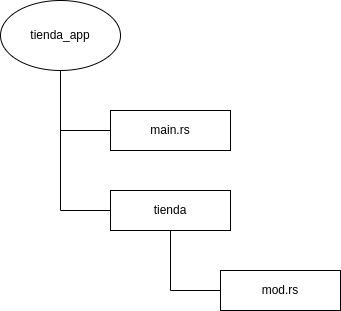
\includegraphics[width=0.5\textwidth]{capitulo1/estructura_basica.png}
	\caption{Estructura básica de programa}
	\label{cap1:001}
\end{figure} 

Con esto, estamos listos para comenzar a construir nuestras estructuras de tareas para poder importarlas y usarlas en la función principal.

\section{Construyendo la estructura de la \textbf{tienda}}

En este momento, tenemos dos tipos diferentes de elementos pendientes: un elemento pendiente y un elemento terminado. Ambos tendrán los mismos atributos, título y estado. Sin embargo, como recordamos con las características, sería ventajoso para nosotros tener dos estructuras diferentes, ya que queremos la máxima flexibilidad para definir la funcionalidad de cada tipo de elemento.

También es posible que deseemos agregar un tipo de elemento de tarea diferente en el futuro. Debido a esto, es lógico tener una estructura base que contenga los atributos comunes y luego dos estructuras que hereden la estructura base: una para el elemento pendiente y otra para el elemento terminado. Para lograr esto, necesitamos la siguiente estructura de directorios en nuestro módulo:

\begin{figure}[htb]
	\centering
	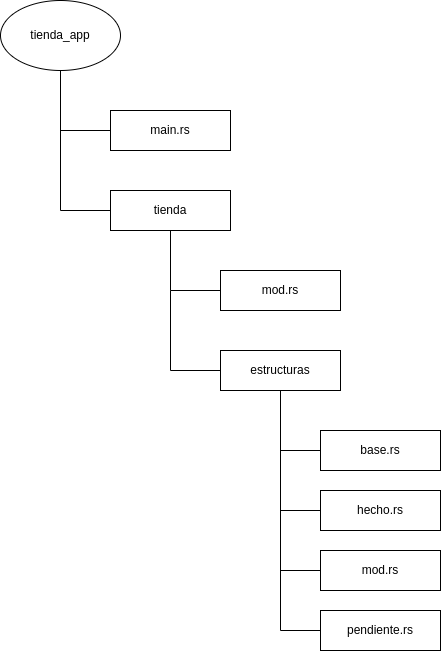
\includegraphics[width=0.4\textwidth]{capitulo1/estructura_tienda.png}
	\caption{Estructura básica de la tienda}
	\label{cap1:002}
\end{figure} 

Podemos ver que hemos creado otro directorio, \textbf{estructuras}, y hemos alojado todas nuestras estructuras allí. En \textbf{base.rs}, definimos la estructura base:

\begin{lstlisting}[language=bash]
pub struct Base{
	pub titulo: String,
	pub estatus: String
}
impl Base {
	pub fn nuevo(titulo_entrada: &str, estatus_entrada: &str) -> Base {
		return Base {titulo: titulo_entrada.to_string(),
			estatus: estatus_entrada.to_string()}
	}
}
\end{lstlisting}

Aquí tenemos una estructura estándar con un constructor. También debemos tener en cuenta que hay una palabra clave \textbf{pub} antes de las definiciones de función, estructura y atributo. Esto se debe a que nuestro objetivo es utilizar esta estructura fuera del archivo. Si no los declaráramos como públicos, el compilador se negaría a compilar si los usáramos externamente.

Ahora que lo hemos definido como público, tenemos que declararlo en nuestro archivo \textbf{tienda\_app/estructuras/mod.rs}:

\begin{lstlisting}[language=bash]
mod base
\end{lstlisting}

Esto permite que otros archivos dentro del módulo accedan al archivo base. Sin embargo, debido a que solo queremos que nuestra estructura base se use dentro del módulo, no la hacemos pública.

Queremos usar nuestra estructura base dentro del módulo pero no externamente. Ahora que hemos hecho que nuestra clase base sea accesible para el resto del módulo, podemos definir nuestro elemento de tarea pendiente en el archivo \textbf{hecho.rs}:

\begin{lstlisting}[language=bash]
user super::base::Base;

pub struct Hecho{
	pub super_estructura: Base
}
impl Hecho {
	pub fn nuevo(titulo_entrada: &str) -> Hecho {
		let base: Base = Base::nuevo(titulo_entrada, "hecho");
		return Hecho{super_estructura: base}
	}
}
\end{lstlisting}

Aquí, accedemos a la estructura base a través del archivo tienda/estructuras/mod.rs usando \textbf{super} en la línea de importación en la parte superior del archivo. También bloqueamos el estado en el constructor (la nueva función) y construimos nuestra estructura base con esto. Hacemos esto para asegurarnos de que una estructura Terminada no defina otro estado aparte de Terminado.

Hacemos lo mismo para nuestro elemento de tarea pendiente en nuestro archivo \textbf{pendiente.rs}:

\begin{lstlisting}[language=bash]
use super::base::Base;

pub struct Pendiente{
	pub super_estructura: Base
}
impl Pendiente{
	pub fn nuevo(titulo_entrada: &str) -> Pendiente {
		let base: Base = Base::nuevo(titulo_entrada, "pendiente");
		return Pendiente{super_estructura: base}
	}
}
\end{lstlisting}


Ahora que tenemos las estructuras que necesitamos, podemos definirlas públicamente en nuestro archivo tienda/estructuras/mod.rs para permitir que el archivo principal las use:

\begin{lstlisting}[language=bash]
mod base
pub mod hecho
pub mod pendiente
\end{lstlisting}

Ahora que nuestras estructuras están listas, podemos hacer que estén disponibles, definiéndolas públicamente en el archivo \textbf{tienda/mod.rs}:

\begin{lstlisting}[language=bash]
pub mod estructuras;
\end{lstlisting}


Ahora nuestro módulo está listo para usar en la función principal con lo siguiente:

\begin{lstlisting}[language=bash]
mod tienda;

use tienda::estructuras::hecho::Hecho;
use tienda::estructuras::pendiente::Pendiente;

fn main() {
	let hecho: Hecho = Hecho::nuevo("shopping");
	println!("{}", hecho.super_struct.titulo);
	println!("{}", hecho.super_struct.estatus);
}
\end{lstlisting}

Aquí tenemos una estructura estándar con un constructor. También debemos tener en cuenta que hay una palabra clave \textbf{pub} antes de las definiciones de función, estructura y atributo. Esto se debe a que nuestro objetivo es utilizar esta estructura fuera del archivo. Si no los declaráramos como públicos, el compilador se negaría a compilar si los usáramos externamente.

Ahora que lo hemos definido como público, tenemos que declararlo en nuestro archivo tienda/estructuras/mod.rs:

\begin{lstlisting}[language=bash]
mod base;	
\end{lstlisting}

Esto permite que otros archivos dentro del módulo accedan al archivo base. Sin embargo, debido a que solo queremos que nuestra estructura base se use dentro del módulo, no la hacemos pública.

Queremos usar nuestra estructura base dentro del módulo pero no externamente. Ahora que hemos hecho que nuestra clase base sea accesible para el resto del módulo, podemos definir nuestro elemento de tarea pendiente en el archivo hecho.rs:

\begin{lstlisting}[language=bash]
use super::base::Base;

pub struct Hecho {
	pub super_struct: Base	
}
impl Hecho {
	pub fn new(input_title: &str) -> Hecho {
		let base: Base = Base::nuevo(input_title,
		"done");
		return Hecho{super_struct: base}	
	}	
}	
\end{lstlisting}

Aquí, accedemos a la estructura base a través del archivo \textbf{tienda/estructuras/mod.rs} usando \textbf{super} en la línea de importación en la parte superior del archivo. También bloqueamos el estado en el constructor (la nueva función) y construimos nuestra estructura base con esto. Hacemos esto para asegurarnos de que una estructura \textbf{Terminada} no defina otro estado aparte de \textbf{Terminado}.

Hacemos lo mismo para nuestro elemento de tarea pendiente en nuestro archivo \textbf{pendiente.rs}:

\begin{lstlisting}[language=bash]
use super::base::Base;

pub struct Pendiente{
	pub super_estructura: Base
}
impl Pendiente{
	pub fn nuevo(titulo_entrada: &str) -> Pendiente {
		let base: Base = Base::nuevo(titulo_entrada, "pendiente");
		return Pendiente{super_estructura: base}
	}
}	
\end{lstlisting}

Ahora que tenemos las estructuras que necesitamos, podemos definirlas públicamente en nuestro archivo \textbf{tienda/estructuras/mod.rs} para permitir que el archivo principal las use:

\begin{lstlisting}[language=bash]
mod base;
pub mod hecho;
pub mod pendiente;
\end{lstlisting}

Ahora que nuestras estructuras están listas, podemos hacer que estén disponibles definiéndolas públicamente en el archivo \textbf{tienda/mod.rs}:

\begin{lstlisting}[language=bash]
pub mod estructuras;
\end{lstlisting}

Ahora nuestro módulo está listo para usar en la función principal con lo siguiente:

\begin{lstlisting}[language=bash]
mod tienda;

use tienda::estructuras::hecho::Hecho;
use tienda::estructuras::pendiente::Pendiente;


fn main() {
	let hecho: Hecho = Hecho::nuevo("Comprando");
	println!("{}", hecho.super_estructura.titulo);
	println!("{}", hecho.super_estructura.estatus);
	let pendiente: Pendiente = Pendiente::nuevo("Lavandaria");
	println!("{}", pendiente.super_estructura.titulo);
	println!("{}", pendiente.super_estructura.estatus);
}
\end{lstlisting}

Aquí, podemos ver que definimos nuestro módulo y luego importamos las dos estructuras que queremos usar. Luego los definimos y luego los imprimimos.

Esto es útil, sin embargo, a medida que el programa crece, podríamos terminar con largas listas de importación a medida que importamos cada estructura pública que alberga el módulo. Esto tampoco es escalable. Si necesitáramos usar nuestro módulo en otro módulo, también tendríamos que reescribir muchas importaciones. Otros desarrolladores también podrían implementar nuestro módulo de forma incorrecta. Para evitar que ocurran estos problemas, podemos construir una interfaz. Vamos a discutir esto más en la siguiente sección.

\section{Manejando estructuras con fábricas}

Podemos construir nuestra interfaz con el patrón de fábrica. Aquí es donde seleccionamos la estructura correcta en función de la entrada, la construimos y la devolvemos. Esto se puede hacer en el archivo \textbf{tienda/mod.rs}:


\begin{lstlisting}[language=bash]
pub mod estructuras;

use estructuras::hecho::Hecho;
use estructuras::pendiente::Pendiente;

pub enum TiposItem {
	Pendiente(Pendiente),
	Hecho(Hecho)
}
pub fn fabrica_tienda(tipo_item: &str, titulo_item: &str) -> Result<TiposItem, &'static str> {
	if tipo_item == "pendiente" {
		let item_pendiente = Pendiente::nuevo(titulo_item);
		Ok(TiposItem::Pendiente(item_pendiente))
	}
	else if tipo_item == "hecho" {
		let item_hecho = Hecho::nuevo(titulo_item);
		Ok(TiposItem::Hecho(item_hecho))
	}
	else {
		Err("Esto no es aceptado")
	}
}
\end{lstlisting}

Aquí, bloqueamos las estructuras eliminando la definición de publicación, ya que solo permitiremos que se use a través de la interfaz, que es la función \textbf{fabrica\_tienda}. En esta función, verificamos el tipo de entrada y construimos la estructura según ese tipo. También empaquetamos un error si pasamos un tipo que no tenemos. También podemos ver que hemos utilizado una enumeración para habilitar la devolución de los dos tipos de elementos.

En este punto, hay una oportunidad de refactorización. Se podría argumentar que solo necesitábamos una estructura y que el tipo podía manejarse en la fábrica, reduciendo la necesidad de múltiples estructuras. Esta es una observación verdadera. Sin embargo, planeamos comenzar a agregar características a nuestras estructuras. En este momento, las estructuras múltiples pueden parecer un poco excesivas, pero debemos mantener la flexibilidad en nuestro código.

Ahora que nuestra interfaz está definida, podemos utilizar esto en la función principal llamando a la fábrica con algunos parámetros y usando una declaración de coincidencia:

\begin{lstlisting}[language=bash]
mod tienda;
use tienda::TiposItem;
use tienda::fabrica_tienda;

fn main() {
	let tienda_item: Result<TiposItem, &'static str> = fabrica_tienda("pendiente", "hacer");
	match tienda_item.unwrap() {
		TiposItem::Pendiente(item) => println!("Esto es un item pendiente con titulo: {}", item.super_estructura.titulo),
		TiposItem::Hecho(item) => println!("Esto es un item hecho con titulo: {}", item.super_estructura.titulo)
	} 
}	
\end{lstlisting}

Esto puede parecer excesivo por ahora: la simple verificación de parámetros y la obtención de la estructura podrían haberse realizado en la función principal. Sin embargo, a medida que crece la complejidad, \textbf{main} se volverá inmanejable. Es mejor mantener la lógica que rodea la definición y la construcción de tareas pendientes en su propio módulo.

En este momento, nuestros elementos de tareas pendientes no hacen nada. Albergan diferentes atributos, pero no pueden eliminar, guardar, actualizar u obtener. Todo lo que pueden hacer son los atributos de la casa. Para definir la funcionalidad, necesitamos darle a nuestras estructuras algunos rasgos.

\section{Definiendo funcionalidad con rasgos (traits)}

Ahora que tenemos nuestros rasgos, es hora de que tengan alguna funcionalidad. Vamos a hacer esto con rasgos. Para escalabilidad y flexibilidad, mantendremos nuestros rasgos tan simples y aislados como sea posible. Definir un rasgo para cada tipo de proceso nos brinda la capacidad de ajustar la funcionalidad para cada tipo.

Para lograr esto, debemos agregar los rasgos del directorio dentro del directorio \textbf{estructuras}. Dentro del directorio de rasgos, tenemos un archivo para cada proceso y un archivo \textbf{mod.rs} para declararlos (ver figura \ref{cap1:003}).

\begin{figure}[htb]
	\centering
	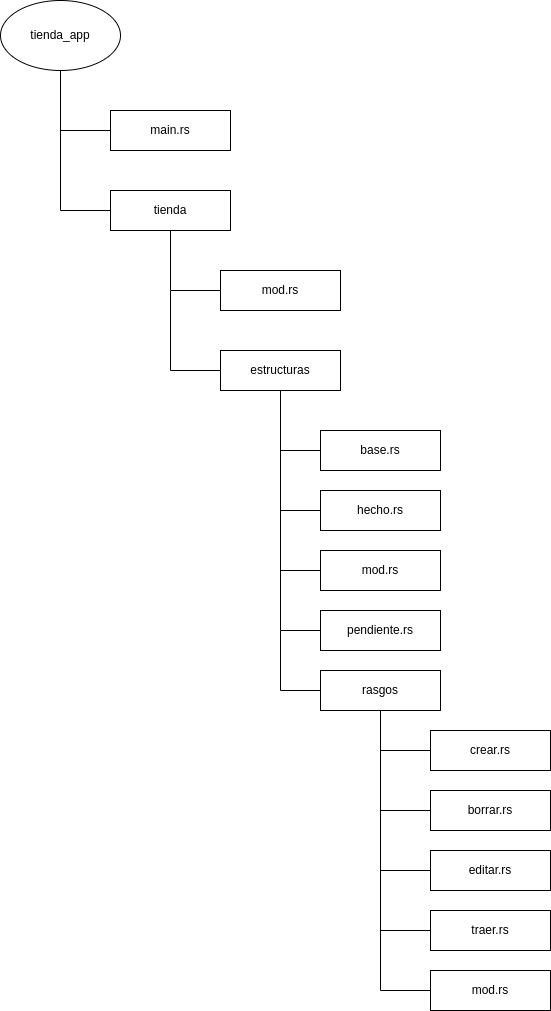
\includegraphics[width=0.4\textwidth]{capitulo1/estructura_tienda2.png}
	\caption{Estructura básica de la tienda con rasgos}
	\label{cap1:003}
\end{figure} 

Primero, definamos funciones que impriman el proceso. Interactuaremos con el entorno de lectura y escritura en un archivo en la siguiente sección. Podemos deducir que las funciones de creación, eliminación, edición y obtención de características requerirán un título. Por lo tanto, en el archivo \textbf{traer}, podemos definir el siguiente rasgo:


\begin{lstlisting}[language=bash]
pub trait Traer {
	fn traer(&self, titulo: &str) {
		println!("{} esta siendo recuperada", titulo);
	}
}	
\end{lstlisting}


Aquí, vinculamos la función \textbf{traer} con el parámetro \textbf{\&self}, que permite que la estructura llame a la función directamente como \textbf{some\_struct.traer(\&String::from("something"))}. También tomamos el título. Nuevamente, por ahora, solo imprimiremos una declaración para garantizar que funcione el mapeo de rasgos en múltiples archivos.

Con el proceso de edición, podemos tener múltiples funciones para diferentes procesos. En este momento, todo lo que necesitamos es una función para configurar un elemento como hecho y otra función para configurar un elemento como pendiente. Podemos definir estos en el archivo \textbf{editar.rs}:

\begin{lstlisting}[language=bash]
pub trait Editar {
	fn ajustar_a_hecho(&self, titulo: &str) {
		println!("{} esta siendo ajustado a hecho", titulo);
	}
	fn ajustar_a_pendiente(&self, titulo: &str) {
		println!("{} esta siendo ajustado a pendiente", titulo);
	}
}	
\end{lstlisting}


En términos de \textbf{Crear}, solo hay una función que necesitamos, que es \textbf{crear}. Esto se puede definir en el archivo \textbf{crear.rs}:

\begin{lstlisting}[language=bash]
pub trait Crear {
	fn crear(&self, titulo: &str) {
		println!("{} esta siendo creado", titulo);
	}
}
\end{lstlisting}

Similar a esto, todo lo que necesitamos es una sola función de eliminación en el rasgo Borrar en el archivo \textbf{borrar.rs}:

\begin{lstlisting}[language=bash]
pub trait Borrar {
	fn borrar(&self, titulo: &str) {
		println!("{} esta siendo borrado", titulo);
	}
}	
\end{lstlisting}

Ahora que tenemos todos nuestros rasgos, tenemos que definirlos públicamente en el archivo mod del directorio de rasgos para que se pueda acceder a ellos desde el exterior:

\begin{lstlisting}[language=bash]
pub mod crear;
pub mod borrar;
pub mod editar;
pub mod traer;
\end{lstlisting}

Ahora que son accesibles, tenemos que hacerlos accesibles para las estructuras definiéndolos públicamente en el archivo \textbf{mod.rs} en el directorio de estructuras:

\begin{lstlisting}[language=bash]
pub mod rasgos;
mod base;
pub mod hecho;
pub mod pendiente;
\end{lstlisting}


Esto permite que nuestras estructuras usen \textbf{super} para acceder a los rasgos. Para la estructura \textbf{Hecho}, debemos permitir que el programa obtenga, edite y elimine implementando estos rasgos en la estructura \textbf{Hecho}:

\begin{lstlisting}[language=bash]
use super::base::Base;
use super::rasgos::traer::Traer;
use super::rasgos::borrar::Borrar;
use super::rasgos::editar::Editar;

pub struct Hecho{
	pub super_estructura: Base
}
impl Hecho {
	pub fn nuevo(titulo_entrada: &str) -> Hecho {
		let estatus_entrada: String = String::from("hecho");
		let base: Base = Base::nuevo(titulo_entrada, "hecho");
		return Hecho{super_estructura: base}
	}
}
impl Traer for Hecho {}
impl Borrar for Hecho {}
impl Editar for Hecho {}
\end{lstlisting}

Para la estructura\textbf{ Pendiente}, vamos a habilitarla para crear, editar, obtener y eliminar:

\begin{lstlisting}[language=bash]
use super::base::Base;
use super::rasgos::crear::Crear;
use super::rasgos::editar::Editar;
use super::rasgos::traer::Traer;
use super::rasgos::borrar::Borrar;

pub struct Pendiente{
	pub super_estructura: Base
}
impl Pendiente{
	pub fn nuevo(titulo_entrada: &str) -> Pendiente {
		let base: Base = Base::nuevo(titulo_entrada, "pendiente");
		return Pendiente{super_estructura: base}
	}
}
impl Crear for Pendiente{}
impl Editar for Pendiente{}
impl Traer for Pendiente{}
impl Borrar for Pendiente{}	
\end{lstlisting}

Ahora que las estructuras están mejoradas con nuestros rasgos, podemos ver cuán escalable es esto. Si añadimos otra estructura de tareas pendientes, podemos colocar una variedad de rasgos para darle instantáneamente la funcionalidad que necesitamos. También podemos eliminar/agregar rasgos de/a nuestras estructuras existentes con facilidad. Esto demuestra el poder que nos dan las estructuras. Ahora que tenemos nuestros rasgos, podemos demostrar cómo se pueden usar en main con lo siguiente:

\begin{lstlisting}[language=bash]
mod tienda;
use tienda::TiposItem;
use tienda::fabrica_tienda;
use tienda::estructuras::rasgos::crear::Crear;

fn main() {
	let tienda_item: Result<TiposItem, &'static str> = fabrica_tienda("pendiente", "lavando");
	match tienda_item.unwrap() {
		TiposItem::Pendiente(item) => item.crear(
		&item.super_estructura.titulo),
		TiposItem::Hecho(item) => println!(
		"Esta hecho el item con titulo: {}",
		item.super_estructura.titulo)	
	}	
}
\end{lstlisting}

Debe tenerse en cuenta que importamos el rasgo Create en main. Aunque el rasgo Crear se implementa para la estructura Pendiente, no podrá activarse si no se importa porque el compilador no lo encontrará.

Lo que hemos hecho aquí es construir nuestro propio módulo, que contiene un punto de entrada. Luego lo importamos a la función principal y lo ejecutamos. Ahora que la estructura básica está construida y funcionando, necesitamos que el módulo interactúe con el entorno pasando variables y escribiendo en un archivo para que sea útil.	


\section{Interacción con el ambiente}

Para interactuar con el entorno, tenemos que manejar dos cosas. Primero, necesitamos cargar, guardar y editar el estado de las tareas pendientes. En segundo lugar, también tenemos que aceptar la entrada del usuario para editar y mostrar datos. Nuestro programa puede lograr esto ejecutando los siguientes pasos para cada proceso:

\begin{itemize}
	\item Recopilar argumentos del usuario.
	\item Defina un comando (obtener, editar, eliminar y crear) y defina un título de tarea a partir de los comandos.
	\item Cargue un archivo \textbf{JSON} que almacene los elementos pendientes de ejecuciones anteriores del programa.
	\item Ejecute una función de obtención, edición, eliminación o creación basada en el comando pasado al programa, guardando el resultado del estado en un archivo \textbf{JSON} al final.
	\item Podemos comenzar a hacer posible este proceso de cuatro pasos cargando inicialmente nuestro estado con la caja de \textbf{serde}.
\end{itemize}

\subsection{Leyendo y escribiendo archivos \textbf{JSON}}

Para instalar el \textbf{crate serde}, definimos la dependencia en el archivo \textbf{Cargo.toml} en la sección [dependencias]:

\begin{lstlisting}[language=bash]
[dependencies]
serde_json = {version = "1.0.79", default-features = false, features = ["alloc"]}
\end{lstlisting}

Para administrar la lectura y escritura en el archivo JSON, tiene sentido crear nuestro propio módulo, ya que habrá varios lugares donde escribiremos datos en el archivo. Sin embargo, el módulo en sí será bastante pequeño y consistirá solo en funciones de lectura y escritura. No sería práctico dedicarle un directorio completo. Podemos crear nuestro propio módulo con solo un archivo en el mismo directorio del archivo principal. En nuestro archivo \textbf{src/estado.rs}, definimos los métodos de lectura y escritura

\begin{lstlisting}[language=bash]
use std::fs::File;
use std::fs;
use std::io::Read;
use serde_json::Map;
use serde_json::value::Value;
use serde_json::json;

pub fn leer_archivo(nombre_archivo: &str) -> Map<String, Value> {
	let mut archivo = File::open(nombre_archivo.to_string()).unwrap();
	let mut datos = String::new();
	archivo.read_to_string(&mut datos).unwrap();
	let json: Value = serde_json::from_str(&datos).unwrap();
	let estado: Map<String, Value> = json.as_object().unwrap().clone();
	return estado
}
\end{lstlisting}

En la función de lectura, tomamos la ruta del archivo como una cadena y usamos la biblioteca estándar para abrirlo. Directamente lo desenvolvemos. Si hay un error aquí, entonces no tiene sentido continuar con el programa. Luego definimos una cadena mutable con el nombre de datos y leemos el archivo en esa cadena (recuerde que las cadenas son referencias a cadenas literales).

Luego usamos \textbf{serde} para convertir esa cadena en un valor JSON y luego definimos ese valor como un objeto y lo clonamos para obtener un mapa \textbf{serde JSON}. Si no lo clonamos, simplemente estaremos devolviendo una referencia. Nos tomamos la molestia de convertirlo en un mapa para obtener la funcionalidad adicional.

Más abajo en el archivo \textbf{src/estado.rs}, definimos el archivo de escritura:

\begin{lstlisting}[language=bash]
pub fn escribir_a_archivo(nombre_archivo: &str, estado: &mut Map<String, Value>) {
	let nuevo_dato = json!(estado);
	fs::write(nombre_archivo.to_string(), nuevo_dato.to_string()).expect("No se pudo escribir el archivo");   
}
\end{lstlisting}	

Aquí, aceptamos la ruta del archivo y el mapa, volvemos a convertir el mapa a JSON usando la macro y luego lo convertimos en una cadena para escribir en el archivo.

Para verificar si esto funciona, debemos importarlo a \textbf{main}, leer un archivo \textbf{JSON}, obtener algunos parámetros del usuario y escribir una nueva entrada en el archivo:

\begin{lstlisting}[language=bash]
mod estado;

use std::env;
use estado::{escribir_a_archivo, leer_archivo};
use serde_json::value::Value;
use serde_json::{Map, json};

fn main() {
	
	let args: Vec<String> = env::args().collect();
	let estatus: &String = &args[1];
	let titulo: &String = &args[2];
	let mut estado: Map<String, Value> = leer_archivo("./estado.json");
	println!("{:?}", estado);
	estado.insert(titulo.to_string(), json!(estatus));
	escribir_a_archivo("./estado.json", &mut estado);
}
\end{lstlisting}

Aquí, recopilamos los argumentos del entorno pasados por el usuario y los recopilamos en un vector de cadenas. Luego definimos los comandos del vector args. Una vez que hayamos hecho eso, cargamos los datos del archivo JSON y los imprimimos usando la notación de depuración. Un resultado de ejemplo (según el contenido del archivo JSON) de esta instrucción de impresión es el siguiente:

\begin{lstlisting}[language=bash]
{"compras": String("pendiente"), "lavado": String("hecho")}
\end{lstlisting}

Luego insertamos la nueva entrada y luego escribimos en un archivo. Nuestra ruta raíz será donde está el archivo \textbf{Cargo.toml}, por lo que definimos un archivo JSON vacío llamado \textbf{estado.json} junto al archivo \textbf{Cargo.toml}. Para permitir que nuestras tareas pendientes interactúen con el estado, debemos habilitar nuestros rasgos de tareas pendientes para manipular el estado.

Se crea el archivo estado.rs con el siguiente contenido:

\begin{lstlisting}[language=bash]
{"lola":"hola","shopping":"pending","washing":"done"}
\end{lstlisting}


\section{Mejorando los rasgos}

Teniendo en cuenta que se ha definido el estado, ahora tenemos una mejor idea de lo que realmente necesitan nuestras funciones de rasgos. Inicialmente podemos comenzar con nuestro rasgo más simple, que es obtener. Aquí, tenemos que obtener un elemento pendiente por el título del estado e imprimirlo. Si no está, imprimimos que el título no estaba en el mapa:

\begin{lstlisting}
use serde_json::Map;
use serde_json::value::Value;

pub trait Traer {
	fn traer(&self, titulo: &str, estado: &Map<String, Value>) {
		let item: Option<&Value> = estado.traer(titulo);
		match item {
			Some(resultado) => {
				println!("\n\nItem: {}", titulo);
				println!("Estatus: {}\n\n", resultado)
			},
			None => println!("item: {} no fue encontrado", titulo)
		}
	}
}		
\end{lstlisting}

Aquí, tomamos el estado, llamamos a la función get para el mapa y luego lo administramos con una declaración de coincidencia e imprimimos el resultado.

El rasgo que podemos abordar es el rasgo Crear. En este rasgo, necesitamos insertar nuestra nueva entrada en el estado y luego usar nuestra función \textbf{escribir\_a\_archivo} para escribir el estado actualizado en el archivo JSON que estamos usando para almacenar nuestros elementos pendientes:

\begin{lstlisting}
use serde_json::Map;
use serde_json::value::Value;
use serde_json::json;
use crate::estado::escribir_a_archivo;
pub trait Crear {
	fn crear(&self, titulo: &str, estatus: &String, estado: &mut Map<String, Value>) {
		estado.insert(titulo.to_string(), json!(estatus));
		escribir_a_archivo("./estado.json", estado);
		println!("{} esta siendo creado", titulo);
	}
}	
\end{lstlisting}

Aquí, podemos ver que usamos el módulo de estado definido en \textbf{\textit{main}} con el comando use \textbf{\textit{crate}}. El rasgo de eliminación tiene el mismo enfoque pero con la función de eliminación se llama en el mapa:

\begin{lstlisting}
use serde_json:.Map;
use serde_json::value::Value;
use crate::estado::escribir_a_archivo;
pub trait Borrar {
	fn borrar(&self, titulo: &str, estado: &mut Map<String, Value>) {
		estado.remove(titulo);
		escribir_a_archivo("./estado.json", estado);
		println!("{} esta siendo borrado", titulo);
	}
}
\end{lstlisting}

Para el rasgo Editar, necesitamos dos funciones: una para establecer una tarea pendiente como pendiente y otra para configurar una tarea pendiente como lista en el estado, como se muestra:

\begin{lstlisting}
use serde_json::Map;
use serde_json::value::Value;
use serde_json::json;
use crate::estado::escribir_a_archivo;
pub trait Editar {
	fn ajustar_a_hecho(&self, titulo: &str, estado:: &mut Map<String, Value>) {
		estado.insert(titulo.to_string(), json!(String::from("hecho")));
		escribir_a_archivo("./estado.json", estado);
		println!("{} esta siendo ajustado a hecho", titulo);
	}
	fn ajustar_a_pendiente(&self, titulo: &str, estado: &mut Map<String, Value>) {
		estado.insert(titulo.to_string(), json!(String::from("pendiente")));
		escribir_a_archivo("./estado.json", estado)
		println!("{} esta siendo ajustado a pendiente", titulo);
	}
}
\end{lstlisting}

Nuestros rasgos ahora pueden interactuar con el archivo JSON y realizar los procesos para los que están destinados. Sin embargo, la simple interacción directa con los rasgos en el archivo principal no es escalable. A medida que el programa crezca, es posible que necesitemos usar estos rasgos en otro lugar. Para protegernos contra esto, podemos crear nuestra propia interfaz para administrar el uso de estos rasgos creando nuestro propio módulo de proceso.

\section{Procesando rasgos y estructuras}

Al igual que nuestro módulo de estado, el módulo de proceso solo necesitará algunas funciones. Por lo tanto, podemos definir el módulo en un archivo \textbf{src/procesos.rs}. El propósito de este módulo es dirigir el flujo de los comandos. Necesitamos un punto de entrada para procesar la entrada y dirigirla a la función correcta para procesar el artículo. En primer lugar, importemos todas las estructuras y rasgos que necesitamos:

\begin{lstlisting}
use serde_json::Map;
use serde_json::value::Value;
use super::tienda::TiposItem;
use super::tienda::estructuras::hecho::Hecho;
use super::tienda::estructuras::pendiente::pendiente;
use super::tienda::estructuras::rasgos::traer::Traer;
use super::tienda::estructuras::rasgos::crear::Crear;
use super::tienda::estructuras::rasgos::borrar::Borrar;
use super::tienda::estructuras::rasgos::editar::Editar;
\end{lstlisting}

Luego definimos las funciones que nos permiten procesar estructuras Terminadas y Pendientes:

\begin{lstlisting}
fn proceso_pendiente(item: Pendiente, comando: String, estado: &Map<String, Value>) {
	let mut estado = estado.clone();
	match comando.as_str() {
		"traer" =>  item.traer(&item.super_struct.title, &estado),
		"crear" =>  item.crear(&item.super_struct.title, &item.super_struct.status, &mut estado),
		"borrar" => item.borrar(&item.super_struct.title, &mut estado),
		"editar" => item.ajustar_a_hecho(&item.super_struct.title, &mut estado),
		_ => println!("comando: {} no soportado", comando)
		
	}
}
fn proceso_hecho(item: Done, comando: String, estado: &Map<String, Value>) {
	let mut estado = estado.clone();
	match comando.as_str() {
		"traer" => item.traer(&item.super_struct.title, &estado),
		"borrar" => item.borrar(&item.super_struct.title, &mut estado),
		"editar" => item.ajustar_a_pendiente(&item.super_struct.title, &mut estado),
		_ => println!("comando: {} no soportado", comando)
	}
}
\end{lstlisting}

Ahora que hemos definido funciones que procesan nuestras estructuras pendientes, podemos crear un punto de entrada que tome una estructura, un estado de memoria y un comando para que podamos canalizar la estructura hacia la función correcta:

\begin{lstlisting}
pub fn proceso_entrada(item: ItemTypes, comando: String, estado: &Map<String, Value>) {
	match item {
		TiposItem::Pendiente(item) => process_pending(item, comando, estado),
		TiposItem::Hecho(item) => process_done(item, comando, estado)
	}    
}
\end{lstlisting}

Lo que tenemos aquí es esencialmente una declaración de coincidencia que se asigna a otras declaraciones de coincidencia. Esto nos da mucha flexibilidad. Si vamos a agregar un tipo, todo lo que tenemos que hacer es agregar una línea en la declaración de coincidencia de la función proceso\_entrada (nuestro punto de entrada). También podemos agregar declaraciones condicionales adicionales en las funciones. Podemos eliminar y agregar comandos rápidamente porque cualquier cosa agregada que no coincida es capturada por el operador \_.

Cabe señalar que tenemos que importar los rasgos al archivo. Aunque los rasgos han sido implementados por las estructuras en el módulo de tareas pendientes, el archivo que llama al rasgo vinculado a la estructura aún debe importarse para ser reconocido. Esta interfaz se puede pasar por el programa y utilizarse en cualquier lugar. Si otro desarrollador necesita otro punto de entrada donde se procesa una tarea pendiente, entonces sabemos que procesará las tareas pendientes de manera estandarizada.

Ahora que todos los módulos son completamente funcionales y funcionan entre sí, podemos implementarlos en la función principal:

\begin{lstlisting}
mod estado;
mod tienda;
mod procesos;

use std::env;
use estado::leer_archivo;
use serde_json::value::Value;
use serde_json::Map;
use tienda::fabrica_tienda;
use procesos::proceso_entrada;

fn main() {
	let args: Vec<String> = env::args().collect();
	let comando: &String = &args[1];
	let titulo: &String = &args[2];
	let estado: Map<String, Value> = leer_archivo("./estado.json");
	let estatus: String;
	
	match &estado.get(*&titulo) {
		Some(resultado) => {
			estatus = resultado.to_string().replace('\"', "");
		}
		None=> {
			estatus = "pendiente".to_string();
		}
	}
	let item = fabrica_tienda(&estatus, titulo).expect(&estatus);
	proceso_entrada(item, comando.to_string(), &estado);
}
\end{lstlisting}

Aquí, todo lo que hemos aprendido está en exhibición. Obtenemos los argumentos del entorno, definimos los comandos y leemos los datos del archivo JSON para obtener el estado de la lista de tareas pendientes. Luego utilizamos lo que sabemos sobre los ámbitos, definiendo el estado como una cadena fuera del bloque de coincidencia para que podamos confiar en el estado fuera del bloque de coincidencia. En el bloque de coincidencia, hacemos una suposición. Si el elemento no existe en el estado, definimos el estado como pendiente. No tendría sentido crear un nuevo elemento terminado. Luego pasamos el estado a la interfaz o nuestro módulo de tareas pendientes. Finalmente, pasamos nuestra estructura, comando y estado de elementos al punto de entrada de nuestro módulo de proceso.

Ahora que hemos construido nuestra aplicación, podemos probarla completamente a través del siguiente procedimiento:

\begin{lstlisting}
cargo run
\end{lstlisting}

Nuestro programa falla porque el índice está fuera de los límites. Esto se debe a que no pusimos ningún comando. Si ejecutamos lo siguiente:

\begin{lstlisting}
cargo run crear lavando
\end{lstlisting}

Recibimos un mensaje de que se está creando el lavado y nuestro archivo JSON vacío ahora se ve así:

\begin{lstlisting}
{"lavando":"pendiente"}
\end{lstlisting}


Ejecutar el comando \textbf{traer} (\textbf{cargo run traer lavando}) nos da la siguiente impresión:

\begin{lstlisting}
Articulo: lavado
Estado: Pendiente"
\end{lstlisting}


Ejecutando el comando de edición (\textbf{cargo run editar lavando}), obtenemos una impresión que nos dice que el lavado se ha configurado como hecho, y nuestro archivo \textbf{JSON} se ve así:

\begin{lstlisting}
{"lavado":"hecho"}
\end{lstlisting}


Ejecutar el comando de eliminación (\textbf{cargo run borrar lavando}) elimina el elemento de lavado en el archivo \textbf{JSON}.

Básicamente, lo que hemos hecho aquí es crear un programa que acepte algunas entradas de la línea de comandos, interactúe con un archivo y lo edite según el comando y los datos de ese archivo. Los datos son bastante simples: un título y un estado.

Podríamos haber hecho todo esto en la función principal con múltiples sentencias de coincidencia y bloques if, else if y else. Sin embargo, esto no es escalable. En cambio, construimos estructuras que heredaron otras estructuras, que luego implementaron rasgos. Luego empaquetamos la construcción de estas estructuras en una fábrica que permite que otros archivos usen toda esa funcionalidad en una sola línea de código.

Luego construimos una interfaz de procesamiento para que la entrada de comando, el estado y la estructura pudieran procesarse, lo que nos permitió agregar funcionalidad adicional y cambiar el flujo del proceso con unas pocas líneas de código. Nuestra función principal solo tiene que centrarse en recopilar los argumentos de la línea de comandos y coordinar cuándo llamar a las interfaces del módulo. Ahora hemos explorado y utilizado cómo Rust administra los módulos, brindándonos los componentes básicos para crear programas del mundo real que pueden resolver problemas y agregar funciones sin verse perjudicados por la deuda tecnológica y una función principal creciente. Ahora que podemos hacer esto, estamos listos para comenzar a crear aplicaciones web escalables que pueden crecer.

En el próximo capítulo, aprenderemos sobre el marco web Actix para poner en funcionamiento un servidor web básico.